\documentclass[a4paper,11pt]{article}

\usepackage[utf8]{inputenc}
\usepackage[T1]{fontenc}

\usepackage{makeidx}
\usepackage{color}
\usepackage{graphicx}
\usepackage{float}
\usepackage[hidelinks]{hyperref} 
\usepackage{geometry}
\usepackage{fancyhdr}
\usepackage{amsmath}
\usepackage{empheq}
\usepackage{array}
\usepackage{multicol}
\usepackage{csquotes}
\usepackage{listings}
\usepackage{xcolor}

\definecolor{ligthyellow}{RGB}{250,247,220}
\definecolor{darkblue}{RGB}{5,10,85}
\definecolor{ligthblue}{RGB}{1,147,128}
\definecolor{darkgreen}{RGB}{8,120,51}
\definecolor{darkred}{RGB}{160,0,0}
\definecolor{ivi}{RGB}{141,107,185}


\lstset{
    language = scilab,
    captionpos = b,
    extendedchars = true,
    frame = lines,
    numbers = left,
    numberstyle = \tiny,
    numbersep = 5pt,
    keepspaces = true,
    breaklines = true,
    showspaces = false,
    showstringspaces = false,
    breakatwhitespace = false,
    stepnumber = 1,
    showtabs = false,
    tabsize = 3,
    basicstyle = \small\ttfamily,
    backgroundcolor = \color{ligthyellow},
    keywordstyle = \color{ligthblue},
    morekeywords = {include, printf, uchar},
    identifierstyle = \color{darkblue},
    commentstyle = \color{darkgreen},
    stringstyle = \color{darkred},
}

\setlength{\headheight}{15pt}

\setcounter{secnumdepth}{3}
\setcounter{tocdepth}{2}

\makeatletter
\@addtoreset{chapter}{part}
\makeatother 

\hypersetup{
  colorlinks = true,
  breaklinks = true,
  urlcolor = blue,
  linkcolor = black,
  citecolor = green
}

\title{
  \noindent\hrulefill \\
  \vspace{10mm} Compte-rendu TP1 VisA: Callibration de caméra
}

\title{TP VisA, Algorithmes de type FCM appliqués à l'imagerie couleur}
\author{Tristan Camus et Arnaud Cojez}
\date{}

\definecolor{myColor}{rgb}{0.5, 0.1, 0.75}


\begin{document}


\maketitle

\noindent\hrulefill \\

\section{Introduction}

Poursuivant nos travaux sur la logique floue, nous allons dans ce TP segmenter des images.
Alors que l'algorithme du C-Means est déjà fortement utilisé en logique classique, nous allons utiliser différentes variantes de ce dernier, notamment l'algorithme FCM utilisant de la logique floue. Nous tenterons ainsi de segmenter, à l'aide des algorithmes Fuzzy C-Means, Hard C-Means, Possibilistic C-Means et de l'algorithme de Davé, l'image suivante en 6 classes distinctes :

\begin{figure}[H]
\begin{center}
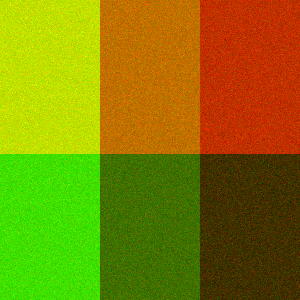
\includegraphics[width=225px]{../img/6_classes_RGB.png}
\end{center}
\caption{Image à segmentée}
\end{figure}

\clearpage

\section{Algorithme FCM}
Fuzzy C-Means est la variante floue la plus simpliste de C-Means. Les résultats de cet algorithme dépendent de la position des centroides calculés aléatoirement au début de l'éxécution. Ainsi, les résultats peuvent varier d'une tentative de classification à une autre. Nous montrons ici des exemples de bons résultats à l'aide de FCM. \\

Ainsi, pour les paramètres suivants : 

\begin{table}[H]
  \begin{center}
    \begin{tabular}{|l|c|}
      \hline
      Nombre de classes & 6 \\
      \hline
      Valeur de m & 2 \\
      \hline
      Nombre d'itération & 100 \\
      \hline
      \shortstack{ Valeur de seuil \\ de stabilité }  & 0.1 \\
      \hline
      Randomisation & 1 \\
      \hline
    \end{tabular}
    \caption{Paramétres utilisés pour l'algorithme de FCM}
  \end{center}
\end{table}

Nous obtenons l'image suivante :

\begin{figure}[H]
\begin{center}

\includegraphics[width=225px]{../img/FCM.png}
\end{center}
\caption{Image segmentée par FCM}
\end{figure}

Ainsi que la courbe de performance suivante :

\begin{figure}[H]
\begin{center}
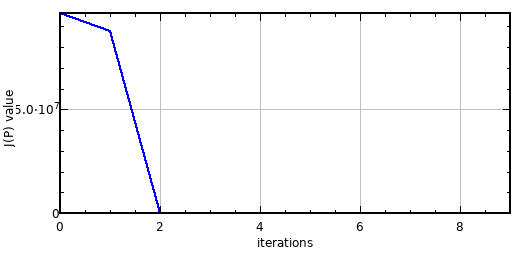
\includegraphics[width=300px]{../img/Perf_FCM.png}
\end{center}
\caption{Courbe de performance pour FCM}
\end{figure}

Le résultat obtenu est assez satisfaisant. On peut distinguer les 6 classes. On note cependant que des points parasites de certaines classes se trouvent dans d'autres.

\section{Algorithme HCM}
Nous avons ensuite utilisé l'algorithme Hard C-Means afin de segmenter l'image. Les résultats de cet algorithme dépendent de la position des centroides calculés aléatoirement au début de l'éxécution. Ainsi, les résultats peuvent varier d'une tentative de classification à une autre. Nous montrons ici des exemples de bons résultats à l'aide de HCM. \\

Ainsi, pour les paramètres suivants : 

\begin{table}[H]
  \begin{center}
    \begin{tabular}{|l|c|}
      \hline
      Nombre de classes & 6 \\
      \hline
      Valeur de m & 1 \\
      \hline
      Nombre d'itération & 100 \\
      \hline
      \shortstack{ Valeur de seuil \\ de stabilité }  & 0.01 \\
      \hline
      Randomisation & 1 \\
      \hline
    \end{tabular}
    \caption{Paramétres utilisés pour l'algorithme de HCM}
  \end{center}
\end{table}

Nous obtenons l'image suivante :

\begin{figure}[H]
\begin{center}
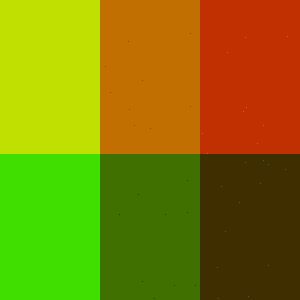
\includegraphics[width=225px]{../img/HCM.png}
\end{center}
\caption{Image segmentée par HCM}
\end{figure}

Ainsi que la courbe de performance suivante :

\begin{figure}[H]
\begin{center}
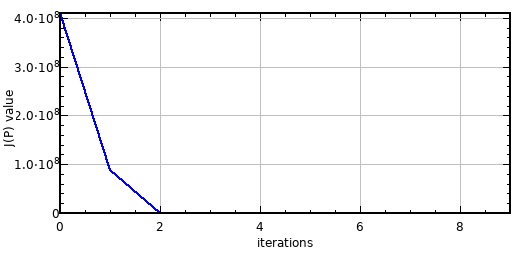
\includegraphics[width=300px]{../img/Perf_HCM.png}
\end{center}
\caption{Courbe de performance pour HCM}
\end{figure}

Le résultat obtenu est assez satisfaisant. On peut distinguer les 6 classes. Cependant, cette image présente plus ou moins les même problème qu'avec FCM et, elle est un exemple de bon résultat. Bien souvent, les deux classes inférieurs droites ne forment qu'une seule classe verte foncée. L'algorithme est aussi plus long à s'éxécuter. 

\section{Algorithme PCM}
Nous avons ensuite utilisé l'algorithme Possibilistic C-Means afin de segmenter l'image. Les résultats de cet algorithme dépendent de la position des centroides calculés aléatoirement au début de l'éxécution. Ainsi, les résultats peuvent varier d'une tentative de classification à une autre. Nous montrons ici des exemples de bons résultats à l'aide de PCM. \\

Ainsi, pour les paramètres suivants : 

\begin{table}[H]
  \begin{center}
    \begin{tabular}{|l|c|}
      \hline
      Nombre de classes & 6 \\
      \hline
      Valeur de m & 2 \\
      \hline
      Nombre d'itération & 40 \\
      \hline
      \shortstack{ Valeur de seuil \\ de stabilité }  & 0.001 \\
      \hline
      Randomisation & 1 \\
      \hline
    \end{tabular}
    \caption{Paramétres utilisés pour l'algorithme de PCM}
  \end{center}
\end{table}

Nous obtenons l'image suivante :

\begin{figure}[H]
\begin{center}

\includegraphics[width=225px]{../img/PCM.png}
\end{center}
\caption{Image segmentée par PCM}
\end{figure}

Ainsi que la courbe de performance suivante :

\begin{figure}[H]
\begin{center}
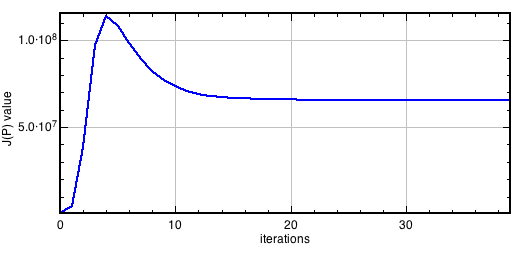
\includegraphics[width=300px]{../img/Perf_PCM.png}
\end{center}
\caption{Courbe de performance pour PCM}
\end{figure}

Le résultat est plutôt mauvais. On ne peut distinguer que 4 classes. les classes de gauches n'en forment que deux, une orange et une verte. C'est encore un fois un exemple. C'est parfois d'autres classes qui ont ce problème. 

\section{Algorithme de Davé}
Nous avons ensuite utilisé l'algorithme de Davé afin de segmenter l'image. Les résultats de cet algorithme dépendent de la position des centroides calculés aléatoirement au début de l'éxécution. Ainsi, les résultats peuvent varier d'une tentative de classification à une autre. Nous montrons ici des exemples de bons résultats à l'aide de l'algorithme de Davé. \\

Ainsi, pour les paramètres suivants : 

\begin{table}[H]
  \begin{center}
    \begin{tabular}{|l|c|}
      \hline
      Nombre de classes & 6 \\
      \hline
      Valeur de m & 2 \\
      \hline
      Nombre d'itération & 100 \\
      \hline
      \shortstack{ Valeur de seuil \\ de stabilité }  & 0.000001 \\
      \hline
      \shortstack{ Valeur du ratio \\ d'aberration }  & 25 \\
      \hline
      Randomisation & 1 \\
      \hline
    \end{tabular}
    \caption{Paramétres utilisés pour l'algorithme de Davé}
  \end{center}
\end{table}

Nous obtenons l'image suivante :

\begin{figure}[H]
\begin{center}
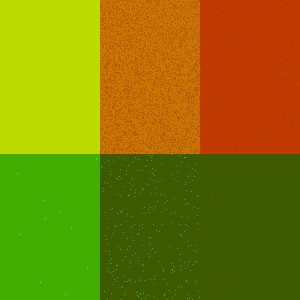
\includegraphics[width=225px]{../img/Dave.png}
\end{center}
\caption{Image segmentée par l'algorithme de Davé}
\end{figure}

Ainsi que la courbe de performance suivante :

\begin{figure}[H]
\begin{center}
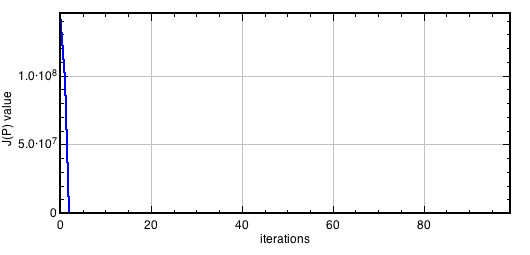
\includegraphics[width=300px]{../img/Perf_Dave.png}
\end{center}
\caption{Courbe de performance pour l'algorithme de Davé}
\end{figure}

Le résultat obtenu est encore une fois assez mauvais. On peut distinguer les 5 classes mais la classe en haut au milieu est fortement parasitée. Encore un fois les résultats changent beaucoup en fonction de la position initiale des centroides. Peut être qu'en trouvant une meilleure valeur pour le ratio d'aberrations, on pourrait obtenir de meilleurs résultats.

\clearpage

\section{Conclusion}
Pour conclure, la méthode FCM présente ici des résultats très correctes. Cependant, avec les méthodes vues dans ce TP, nous ne faisons que calculer des degrés d'appartenance et ne segmentons pas véritablement l'image. En effet, il nous faudrait pour cela définir une heuristique prenant en compte la position des pixels dans l'image.

\end{document}